% ===========================================================================
% MODELO DE RELATORIO  ·  ENE0046 Laboratorio de Eletronica  ·  2026/2
%
% Como usar
%   1. Preencha o bloco IDENTIFICACAO logo abaixo.
%   2. Deixe comentados os autores que nao existirem. Um autor fica centralizado,
%      dois dividem a linha, tres ocupam tercos.
%   3. Substitua o texto de cada secao pelo seu. As orientacoes que estao la
%      dizem o que se espera em cada uma.
%   4. Compile com pdflatex duas vezes, ou com latexmk -pdf.
%
% Estrutura
%   Roteiro 1 nao tem bancada: use so a subsecao 4.1 e a 5.1, e compare o calculo
%   analitico com a simulacao de projeto.
%   Roteiros 2 a 7 usam a estrutura inteira.
%
% O arquivo estilo-relatorio.tex e a imagem logo-unb.png devem estar na mesma
% pasta deste arquivo.
% ===========================================================================
\documentclass[11pt,a4paper]{article}
% !TeX root = modelo-relatorio.tex
% Formatacao do relatorio. Compile o modelo-relatorio.tex, nao este arquivo.
\usepackage[T1]{fontenc}
\usepackage[utf8]{inputenc}
\usepackage[brazil]{babel}
\usepackage[a4paper,top=1.6cm,bottom=1.8cm,left=2.1cm,right=2.1cm]{geometry}
\usepackage[default]{lato}
\usepackage{amsmath,amssymb}
\usepackage{siunitx}
\usepackage{graphicx}
\usepackage{booktabs,array,longtable,colortbl}
\usepackage{enumitem}
\usepackage{tcolorbox}
\usepackage{xcolor}
\usepackage{tikz}
\usepackage{titlesec}
\usepackage{fancyhdr}
\usepackage{caption}
\usepackage{etoolbox}
\usepackage[colorlinks=true,linkcolor=azul,urlcolor=azul,citecolor=azul]{hyperref}
\tcbuselibrary{skins,breakable}

\definecolor{azul}{HTML}{0A4B8C}
\definecolor{azulclaro}{HTML}{E8F0F8}
\definecolor{verde}{HTML}{0B7A4B}
\definecolor{cinza}{HTML}{5B6672}
\definecolor{cinzaclaro}{HTML}{F4F6F8}
\definecolor{vinho}{HTML}{B04A4A}
\definecolor{vinhoclaro}{HTML}{FBF2F2}

\sisetup{output-decimal-marker={,}, per-mode=symbol}
\setlength{\parindent}{0pt}
\setlength{\parskip}{6pt plus 1pt}
\setlist{itemsep=3pt, topsep=4pt, parsep=0pt, leftmargin=1.3em}
\renewcommand{\arraystretch}{1.25}
\linespread{1.06}

% ---- secoes numeradas com marcador colorido -------------------------------
\titleformat{\section}[hang]
  {\Large\bfseries\color{azul}}
  {\raisebox{-1pt}{\tikz\node[fill=azul,text=white,rounded corners=2pt,
     inner sep=3pt,minimum width=20pt,align=center]{\bfseries\thesection};}}
  {10pt}{}
\titlespacing*{\section}{0pt}{16pt plus 3pt}{6pt}
\titleformat{\subsection}{\large\bfseries\color{cinza}}{\thesubsection}{8pt}{}
\titlespacing*{\subsection}{0pt}{11pt plus 2pt}{3pt}

% ---- legendas -------------------------------------------------------------
\captionsetup{font=small,labelfont={bf,color=azul},labelsep=period,skip=6pt}

% ---- identificacao --------------------------------------------------------
\newcommand{\autorA}{}\newcommand{\matA}{}
\newcommand{\autorB}{}\newcommand{\matB}{}
\newcommand{\autorC}{}\newcommand{\matC}{}
\newcommand{\autorum}[2]{\renewcommand{\autorA}{#1}\renewcommand{\matA}{#2}}
\newcommand{\autordois}[2]{\renewcommand{\autorB}{#1}\renewcommand{\matB}{#2}}
\newcommand{\autortres}[2]{\renewcommand{\autorC}{#1}\renewcommand{\matC}{#2}}

\newcommand{\disciplina}{ENE0046 · Laboratório de Eletrônica}
\newcommand{\semestre}{2026/2}
\newcommand{\turma}{}
\newcommand{\roteironum}{}
\newcommand{\roteirotema}{}
\newcommand{\aturma}[1]{\renewcommand{\turma}{#1}}
\newcommand{\roteiro}[2]{\renewcommand{\roteironum}{#1}\renewcommand{\roteirotema}{#2}}

\newcommand{\umautor}[2]{%
  \begin{minipage}[t]{\dimexpr\linewidth-4pt\relax}\centering
    \parbox[t][30pt][t]{\linewidth}{\centering
      {\fontsize{10.5}{12.5}\selectfont #1}}\\[-2pt]
    {\color{cinza}\fontsize{9}{11}\selectfont\texttt{#2}}
  \end{minipage}}

\newcounter{nautores}
\newcommand{\blocoautores}{%
  \setcounter{nautores}{0}%
  \ifdefempty{\autorA}{}{\stepcounter{nautores}}%
  \ifdefempty{\autorB}{}{\stepcounter{nautores}}%
  \ifdefempty{\autorC}{}{\stepcounter{nautores}}%
  \ifnum\value{nautores}=0
    \begin{center}\color{vinho}\bfseries
      Preencha ao menos um autor no preâmbulo do arquivo.
    \end{center}
  \else
    \begin{center}
    \ifcase\value{nautores}\or
      % --- um autor: ocupa o centro
      \begin{minipage}{0.5\textwidth}\umautor{\autorA}{\matA}\end{minipage}%
    \or
      % --- dois autores: metades
      \begin{minipage}{0.42\textwidth}\umautor{\autorA}{\matA}\end{minipage}\hspace{0.04\textwidth}%
      \begin{minipage}{0.42\textwidth}\umautor{\autorB}{\matB}\end{minipage}%
    \or
      % --- tres autores: tercos
      \begin{minipage}{0.31\textwidth}\umautor{\autorA}{\matA}\end{minipage}\hspace{0.015\textwidth}%
      \begin{minipage}{0.31\textwidth}\umautor{\autorB}{\matB}\end{minipage}\hspace{0.015\textwidth}%
      \begin{minipage}{0.31\textwidth}\umautor{\autorC}{\matC}\end{minipage}%
    \fi
    \end{center}
  \fi}

% ---- cabecalho do relatorio -----------------------------------------------
\newcommand{\capa}{%
\begin{tcolorbox}[colback=azul,colframe=azul,boxrule=0pt,arc=4pt,
  left=16pt,right=16pt,top=13pt,bottom=13pt]
\color{white}
\begin{minipage}{0.76\textwidth}
  {\fontsize{9}{11}\selectfont\textbf{\MakeUppercase{\disciplina{} · \semestre{}}}}\\[6pt]
  {\fontsize{22}{25}\selectfont\bfseries Relatório do Roteiro \roteironum}\\[3pt]
  {\fontsize{12.5}{15}\selectfont \roteirotema}
\end{minipage}\hfill
\begin{minipage}{0.2\textwidth}\raggedleft
  \colorbox{white}{\hspace{2pt}\raisebox{-2pt}{
\includegraphics[height=30pt]{logo-unb.png}}\hspace{2pt}}
\end{minipage}
\end{tcolorbox}
\vspace{10pt}
\blocoautores
\ifdefempty{\turma}{}{%
  \begin{center}{\color{cinza}\fontsize{9}{11}\selectfont Turma \turma}\end{center}}
\vspace{4pt}
{\color{azulclaro}\hrule height 2pt}
\vspace{2pt}}

% ---- caixas auxiliares ----------------------------------------------------
\newtcolorbox{formula}{colback=azulclaro,colframe=azul,boxrule=0.8pt,arc=3pt,
  left=12pt,right=12pt,top=9pt,bottom=9pt}
\newtcolorbox{nota}[1]{colback=cinzaclaro,colframe=cinza,boxrule=0.8pt,arc=3pt,
  left=10pt,right=10pt,top=7pt,bottom=7pt,
  title={\textbf{#1}},fonttitle=\small\bfseries,coltitle=white,colbacktitle=cinza}
\newenvironment{resumo}
  {\vspace{6pt}\begin{center}\begin{minipage}{0.92\textwidth}
   \begin{tcolorbox}[colback=cinzaclaro,colframe=cinzaclaro,boxrule=0pt,arc=3pt,
     left=14pt,right=14pt,top=10pt,bottom=10pt,
     borderline west={2.5pt}{0pt}{azul}]
   {\color{azul}\fontsize{8}{10}\selectfont\textbf{RESUMO}}\\[4pt]
   \small}
  {\end{tcolorbox}\end{minipage}\end{center}\vspace{2pt}}

\newtcolorbox{espec}{colback=azulclaro,colframe=azul,boxrule=0.8pt,arc=3pt,
  left=12pt,right=12pt,top=9pt,bottom=9pt,
  title={\textbf{Especificação da matrícula}},fonttitle=\bfseries,
  coltitle=white,colbacktitle=azul}

% ---- rodape ---------------------------------------------------------------
\pagestyle{fancy}\fancyhf{}
\renewcommand{\headrulewidth}{0pt}
\renewcommand{\footrulewidth}{0.4pt}
\fancyfoot[L]{\color{cinza}\fontsize{8}{10}\selectfont \disciplina{} · \semestre{} · Roteiro \roteironum}
\fancyfoot[R]{\color{cinza}\fontsize{8}{10}\selectfont \thepage}

\newlist{referencias}{itemize}{1}
\setlist[referencias]{label={}, leftmargin=1.1em, itemindent=-1.1em,
                     itemsep=3pt, topsep=2pt, parsep=0pt}

\newcommand{\mat}[1]{\texttt{\textbf{#1}}}

\usepackage{float}

% --------------------------- IDENTIFICACAO ---------------------------------
\roteiro{5}{Fontes de Alimentação: Retificação e Regulação}
\aturma{01}

\autorum{Bernardo Manciola Lobo}{21/1026486}
\autordois{Enzo Morrone de Azevedo Muniz}{22/1035442}
\autortres{Matheus Vieira Tiveron}{24/1039879}
% ---------------------------------------------------------------------------

\begin{document}
\capa

\begin{resumo}
  Escreva este parágrafo por último, com 100 a 150 palavras. Diga o que você projetou, sob
  qual especificação, o que simulou ou mediu, o principal resultado numérico e a que
  conclusão chegou. Quem ler só este parágrafo deve saber o que você fez e o que encontrou.
\end{resumo}

\section{Introdução}

Um dos grande problemas encontrados durante o desenvolvimento do sistema elétrico foi
como diminuir as perdas energéticas devido a distribuição de energia. Em resumo, a história
mostrou que a distribuição por corrente alternada desperdiça menos energia, se tornando
predominante no mundo. Assim, surgiu um problema: a maioria das aplicações da eletricidade
precisam de corrente contínua para funcionar. Além disso, pode ser necessário um potencial
estável.

Nesse contexto, técnicas de conversão de energia foram desenvolvidas parar resolver este problema,
permitindo a criação de fontes de corrente contínua. Para implementar uma fonte, um pode seguir
vários passos.

Primeiramente, é feito a retificação da onda com o uso de diodos, com isso, a
corrente passa a seguir por uma direção só. Com um diodo só, apenas é possível aproveitar
metade da onda de entrada, porém, com 4 diodos, é possível fazer um retificador de onda completa,
que será implementado neste experimento.

Em segundo, um filtro capacitivo diminui a variação da tensão entre os picos da entrada.
Dessa forma, surge uma grandeza chamada tensão de ripple $V_r$, que é proporcional à capacitância
do capacitor. Assim, a tensão mínima do filtro fica limitada a saída do retificador - $V_r$ e,
simplificadamente, a saída do filtro se assemelha a uma onda de serra.

Por último, para transformar essa onda de serra em uma tensão constante, é usando um circuito de
regulação usando um diodo zenner. O regulador tem como alvo uma tensão menor que a saída do filtro
e consome, propositalmente, toda a tensão que excede este alvo. Isto é possível devido ao funcionamento
do zenner, ele possui uma chamada tensão de ruptura $V_z$. Com ela, a tensão entre os terminais do
zenner fica limitada a $V_z$, pois qualquer tentativa de excedê-la essencialmente faz o zenner
comportar como um circuito aberto.

Com todos esses estágios é possível construir uma fonte de alimentação DC, que é o objetivo deste relatório.
O texto está organizado nas secções: Fundamentação teórica, Especificação e projeto, Metodologia, Simulação e Resultados.

\section{Fundamentação teórica}

Esta seção deduz as expressões usadas no projeto e na análise dos quatro estágios da fonte linear. As hipóteses adotadas são as de diodo ideal, com tensão de condução nula na análise inicial e corrigida depois para a queda real de \SI{0,7}{\volt} do 1N4007, e de capacitor em regime permanente após o primeiro período da rede. Essas hipóteses serão retomadas na Seção~6, onde se verifica em que medida elas se sustentam no circuito real.
 
\subsection{Retificador de meia onda}
 
No retificador de meia onda, o diodo conduz apenas no semiciclo positivo da fonte, quando a tensão da fonte excede a tensão de condução do diodo. A carga recebe um semiciclo da senoide e tensão nula no semiciclo seguinte. O pico da tensão na carga é, portanto,
 
\begin{equation}
V_{o,\text{pico}} = V_p - V_D ,
\label{eq:meia_onda_pico}
\end{equation}
 
em que \(V_p\) é o pico da fonte e \(V_D\) é a queda direta do diodo, da ordem de \SI{0,7}{\volt} para o 1N4007. A diferença entre o pico da fonte e o pico da carga é a queda no diodo, e é ela que explica por que a carga não recebe a tensão plena da fonte.
 
O valor médio da tensão na carga, para meia onda, é a integral do semiciclo positivo dividida pelo período completo:
 
\begin{equation}
V_{o,\text{médio}} = \frac{1}{T} \int_0^{T/2} V_p \sin(\omega t) \, dt = \frac{V_p}{\pi} .
\label{eq:meia_onda_medio}
\end{equation}
 
Esse valor é aproximadamente \(0{,}318 \, V_p\), ou seja, cerca de um terço do pico da fonte.
 
\subsection{Meia onda com filtro capacitivo}
 
Com o capacitor em paralelo com a carga, o diodo conduz apenas nas proximidades do pico, repondo a carga que a carga drenou ao longo do restante do período. Entre picos consecutivos, a tensão decresce de forma aproximadamente linear, e essa queda é o ripple. Quando a descarga é lenta em relação ao período, a corrente na carga é aproximadamente constante e igual a \(I_L\), e o ripple de pico a pico é
 
\begin{equation}
V_r \approx \frac{I_L}{f C} ,
\label{eq:ripple}
\end{equation}
 
em que \(f\) é a frequência de repetição dos picos: \SI{60}{\hertz} em meia onda e \SI{120}{\hertz} em onda completa. Essa expressão é a base do projeto do capacitor: dado um ripple máximo admissível, o capacitor é
 
\begin{equation}
C \geq \frac{I_L}{f \, V_{r,\max}} ,
\label{eq:capacitor}
\end{equation}
 
arredondado para o valor E12 imediatamente superior.
 
A fração do período em que o diodo conduz é pequena quando o capacitor é grande, e o pico da corrente no diodo é muito maior que a corrente média na carga, porque toda a carga drenada ao longo do período é reposta em um intervalo curto. O efeito de aumentar o capacitor em dez vezes é reduzir o ripple na mesma proporção, mas aumentar o pico de corrente no diodo, porque a reposição ocorre em um intervalo ainda menor.
 
\subsection{Ponte retificadora}
 
Na ponte retificadora, nos semiciclos positivos conduzem \(D_1\) e \(D_2\), e nos negativos \(D_3\) e \(D_4\), de modo que a corrente na carga mantém sempre o mesmo sentido. Os picos se repetem a \SI{120}{\hertz}, e o caminho da corrente atravessa dois diodos em série. O pico da tensão na carga é, portanto,
 
\begin{equation}
V_{o,\text{pico}} = V_p - 2 V_D .
\label{eq:ponte_pico}
\end{equation}
 
A diferença entre o pico da fonte e o pico da carga é o dobro da observada na Seção~3.1, porque dois diodos estão em série no caminho da corrente. O valor médio da tensão na carga, para onda completa, é
 
\begin{equation}
V_{o,\text{médio}} = \frac{2 V_p}{\pi} ,
\label{eq:ponte_medio}
\end{equation}
 
que é o dobro do valor médio da meia onda, como esperado, porque a carga recebe um semiciclo a cada meio período, e não a cada período completo.
 
\subsection{Ponte com filtro}
 
Com o capacitor em paralelo com a carga, o ripple é dado pela mesma Equação~\eqref{eq:ripple}, mas com \(f = \SI{120}{\hertz}\), porque os picos se repetem duas vezes por período da rede. O ripple cai à metade em relação à meia onda com o mesmo capacitor, o que é uma das vantagens da ponte. A tensão mínima na saída do filtro, que será usada no projeto do regulador, é
 
\begin{equation}
V_{\min} = V_{o,\text{pico}} - V_r .
\label{eq:vmin}
\end{equation}
 
\subsection{Regulação com zener}
 
Polarizado reversamente além da tensão de ruptura, o zener mantém a tensão entre os seus terminais em \(V_Z\) enquanto houver corrente reversa suficiente. O resistor \(R_S\) absorve a diferença entre a saída do filtro e \(V_Z\), e a corrente que o atravessa se divide entre a carga e o zener. A regulação é perdida quando a saída do filtro cai a ponto de anular a corrente no zener, o que ocorre primeiro no vale do ripple.
 
O projeto de \(R_S\) parte da condição de que, no vale do ripple, ainda circule a corrente mínima no zener \(I_{Z,\min}\):
 
\begin{equation}
R_S = \frac{V_{\min} - V_Z}{I_L + I_{Z,\min}} ,
\label{eq:rs}
\end{equation}
 
arredondado para o valor E12 imediatamente inferior, para garantir que a corrente no zener não fique abaixo do mínimo. A potência dissipada no zener, no pior caso — pico da saída do filtro e carga retirada —, é
 
\begin{equation}
P_Z = V_Z \frac{V_{\max} - V_Z}{R_S} ,
\label{eq:pz}
\end{equation}
 
em que \(V_{\max}\) é o pico da saída do filtro. Essa potência precisa ser comparada com a potência máxima do zener: \SI{250}{\milli\watt} para o BZX84C na simulação e \SI{500}{\milli\watt} para o 1N754 na bancada.
 
O ripple na saída do regulador é atenuado pela ação do zener, que fixa a tensão em \(V_Z\) enquanto conduz. A razão entre o ripple de entrada e o de saída é a rejeição do regulador, que depende da resistência dinâmica do zener e da corrente que o atravessa. Quanto maior a corrente no zener, menor a resistência dinâmica e maior a rejeição, mas maior a potência dissipada. Quando a corrente no zener se anula no vale do ripple, o zener deixa de conduzir e a regulação é perdida naquele trecho do períod

\section{Especificação e Projeto}
 
Esta seção transcreve a especificação da equipe~2 para a montagem em bancada e leva cada parâmetro até o valor de componente comercial. A Seção~3.1 apresenta a especificação da equipe; a Seção~3.2 detalha o projeto do capacitor e do resistor série; e a Seção~3.3 registra os valores medidos dos componentes efetivamente usados na montagem.
 
\subsection{Especificação da equipe 2}
 
A equipe~2 montou a fonte linear com a especificação da Tabela~\ref{tab:equipe_r5}. A fonte é a mesma para todas as equipes: senoide do gerador de \SI{20}{\volt} de pico a pico (\SI{10}{\volt} de pico) em \SI{60}{\hertz}, com o gerador configurado para carga de alta impedância. A tensão regulada é a do zener 1N754, de \SI{6,8}{\volt}, e a carga é o que varia entre as equipes.
 
\begin{table}[h]
\centering
\caption{Especificação da equipe~2 para a bancada.}
\label{tab:equipe_r5}
\begin{tabular}{lc}
\hline
Grandeza & Valor \\
\hline
Carga $R_L$ & \SI{4,7}{\kilo\ohm} \\
$I_L$ em \SI{6,8}{\volt} & \SI{1,4}{\milli\ampere} \\
\hline
\end{tabular}
\end{table}
 
A corrente de carga é calculada a partir da tensão regulada e da carga:
 
\begin{equation}
I_L = \frac{V_Z}{R_L} = \frac{6{,}8}{4{,}7 \times 10^3} = \SI{1,45}{\milli\ampere} .
\label{eq:il_equipe}
\end{equation}
 
O valor de \SI{1,4}{\milli\ampere} da Tabela~\ref{tab:equipe_r5} é o valor aproximado adotado pela equipe, e é o que será usado nas contas seguintes.
 
\subsection{Projeto dos componentes}
 
\subsubsection{Capacitor de filtro}
 
O capacitor de filtro é calculado pela Equação~\eqref{eq:capacitor} do roteiro, com $f = \SI{60}{\hertz}$ e ripple máximo de \SI{1,5}{\volt} de pico a pico, para a meia onda:
 
\begin{equation}
C \geq \frac{I_L}{f \, V_{r,\max}} = \frac{1{,}4 \times 10^{-3}}{60 \cdot 1{,}5} = \SI{15,6}{\micro\farad} .
\label{eq:capacitor_equipe}
\end{equation}
 
O valor E12 imediatamente superior é \SI{22}{\micro\farad}, mas por limitações de disponibilidade no laboratório, adota-se o \SI{47}{\micro\farad}. Com esse capacitor, o ripple previsto cai para
 
\begin{equation}
V_r = \frac{I_L}{f C} = \frac{1{,}4 \times 10^{-3}}{60 \cdot 47 \times 10^{-6}} = \SI{0,496}{\volt} ,
\label{eq:ripple_equipe}
\end{equation}
 
bem abaixo do máximo de \SI{1,5}{\volt}. O capacitor de \SI{4,7}{\micro\farad} também foi usado, na comparação da Seção~3.2 do roteiro, para verificar o efeito de um capacitor dez vezes menor sobre o ripple e sobre o pico de corrente no diodo.
 
\subsubsection{Resistor série do regulador}
 
O resistor série $R_S$ é calculado pela Equação~\eqref{eq:rs} do roteiro, com $I_{Z,\min} = \SI{1}{\milli\ampere}$ e $V_{\min}$ medido na saída do filtro (pico menos ripple). O valor de $V_{\min}$ depende do capacitor adotado e da queda dos diodos da ponte, e precisa ser medido antes de calcular $R_S$. Com o capacitor de \SI{47}{\micro\farad} e a ponte, o pico da saída do filtro é aproximadamente
 
\begin{equation}
V_{o,\text{pico}} = V_p - 2 V_D = 10 - 2 \cdot 0{,}7 = \SI{8,6}{\volt} ,
\label{eq:pico_ponte_equipe}
\end{equation}
 
e a tensão mínima é $V_{\min} = 8{,}6 - 0{,}496 = \SI{8,1}{\volt}$. O resistor série é, então,
 
\begin{equation}
R_S = \frac{V_{\min} - V_Z}{I_L + I_{Z,\min}} = \frac{8{,}1 - 6{,}8}{1{,}4 \times 10^{-3} + 1 \times 10^{-3}} = \frac{1{,}3}{2{,}4 \times 10^{-3}} = \SI{542}{\ohm} .
\label{eq:rs_equipe}
\end{equation}
 
O valor E12 imediatamente inferior é \SI{470}{\ohm}, mas o valor adotado pela equipe foi \SI{462}{\ohm}, que é o valor medido do resistor de \SI{470}{\ohm} usado na montagem. A diferença entre o calculado e o adotado é de \SI{15}{\%}.
 
A potência dissipada no zener, no pior caso (pico da saída do filtro e carga retirada), é
 
\begin{equation}
P_Z = V_Z \frac{V_{\max} - V_Z}{R_S} = 6{,}8 \cdot \frac{8{,}6 - 6{,}8}{462} = 6{,}8 \cdot \frac{1{,}8}{462} = \SI{26,5}{\milli\watt} ,
\label{eq:pz_equipe}
\end{equation}
 
muito abaixo dos \SI{500}{\milli\watt} do 1N754, o que garante que o zener não será danificado mesmo com a carga retirada.
 
\subsection{Componentes medidos da montagem}
 
Antes de inserir cada componente no protoboard, a equipe~2 mediu o valor real com o multímetro. A Tabela~\ref{tab:medidos_r5} registra os valores teóricos, os adotados e o desvio percentual. O desvio é calculado como
 
\begin{equation}
\text{Desvio} = \frac{\text{adotado} - \text{teórico}}{\text{teórico}} \times 100\% .
\label{eq:desvio}
\end{equation}
 
\begin{table}[h]
\centering
\caption{Valores teóricos, adotados e medidos dos componentes da montagem da equipe~2.}
\label{tab:medidos_r5}
\begin{tabular}{@{}lrrr@{}}
\toprule
\textbf{Grandeza} & \textbf{Teórico} & \textbf{Adotado} & \textbf{Desvio} \\
\midrule
Carga $R_L$ & \SI{4,7}{\kilo\ohm} & \SI{4,7}{\kilo\ohm} & 0,0\% \\
Capacitor & \SI{4,7}{\micro\farad} & \SI{4,7}{\micro\farad} & 0,0\% \\
Capacitor & \SI{47}{\micro\farad} & \SI{47}{\micro\farad} & 0,0\% \\
$R_s$ do regulador & \SI{470}{\ohm} & \SI{462}{\ohm} & $-1,7\%$ \\
\bottomrule
\end{tabular}
\end{table}
 
A carga $R_L$ de \SI{4,7}{\kilo\ohm} foi adotada sem desvio porque o valor nominal do resistor já é o valor comercial da série E12. Os capacitores de \SI{4,7}{\micro\farad} e \SI{47}{\micro\farad} também foram adotados sem desvio, porque são os valores disponíveis no laboratório e o projeto já os considera. O resistor série de \SI{470}{\ohm} apresentou um valor medido de \SI{462}{\ohm}, o que corresponde a um desvio de \SI{-1,7}{\%}, compatível com a tolerância típica dos resistores de filme de carbono (\SI{5}{\%}). A escolha do \SI{470}{\ohm} como valor comercial, em vez dos \SI{542}{\ohm} calculados, reduz a corrente no zener, mas mantém a regulação dentro da faixa de operação.

\section{Metodologia}
 
Esta seção descreve os procedimentos adotados na simulação e na bancada, com os parâmetros que permitem repetir cada medida. A Seção~4.1 apresentará a simulação de projeto de cada integrante; a Seção~4.2 descreve a montagem em bancada; e a Seção~4.3 tratará da simulação da montagem com os valores medidos. Todas as medidas de bancada foram feitas com o gerador de funções, o osciloscópio e o multímetro, e o ripple foi lido no canal do osciloscópio em acoplamento AC, com os cursores.

\subsection{Simulação de projeto, uma por integrante}

Cada integrante recebeu uma especificação diferente da própria matrícula, e portanto chegou
a um dimensionamento diferente. Traga aqui \textbf{uma simulação por integrante}, cada uma
com os componentes que aquela pessoa projetou. São elas que mostram se cada projeto cumpre
o que foi pedido.

\subsubsection{Retificador de meia onda}

O primeiro circuito simulado utiliza uma fonte senoidal de \SI{60}{\hertz}, um diodo
retificador 1N4007 e um resistor de carga $R_L$. Durante o semiciclo positivo,
o diodo conduz quando a tensão de entrada supera sua queda direta, permitindo
a circulação de corrente pela carga. No semiciclo negativo, o diodo permanece
reversamente polarizado e a tensão de saída é aproximadamente nula. Como não
há capacitor de filtro nesta etapa, a saída é uma senoide retificada de meia
onda, conforme a Figura~\ref{fig:sim_retificador_meia_onda}.

\begin{figure}[H]
  \centering
  \includegraphics[width=0.95\linewidth]{imagens/ret_meia_onda_simulacao.png}
  \caption{Circuito de retificação de meia onda e tensão de saída no LTspice,
  na simulação inicial com $R_L=\SI{9,1}{\kilo\ohm}$.}
  \label{fig:sim_retificador_meia_onda}
\end{figure}

\textbf{Especificação individual e dimensionamento da carga.}
Para a matrícula 241039879, os algarismos especificados no roteiro são
$AB=24$ e $I=9$. Assim, a amplitude de pico da fonte e a corrente de carga
especificada são
\begin{equation}
V_p=\frac{V_{pp}}{2}=\frac{24}{2}=\SI{12}{\volt},\qquad
I_L=I\cdot\SI{100}{\micro\ampere}=\SI{900}{\micro\ampere}.
\end{equation}

Embora o zener não faça parte do retificador desta seção, sua tensão nominal
serve de referência para definir $R_L$, que será mantido nas etapas seguintes.
De acordo com o critério do roteiro, a tensão de referência é
\begin{equation}
V_{Z,\mathrm{ref}}=\frac{V_p}{\sqrt{2}}=\frac{12}{\sqrt{2}}
=\SI{8,485}{\volt}.
\end{equation}
O modelo disponível mais próximo é o BZX84C8V2, de tensão nominal
$V_Z=\SI{8,2}{\volt}$, cujo desvio em relação à referência é
\begin{equation}
\varepsilon_{V_Z}=\frac{8,2-8,485}{8,485}\cdot100\%
\approx-3,36\%.
\end{equation}
A resistência correspondente à corrente especificada, na tensão nominal
selecionada, resulta em
\begin{equation}
R_{L,\mathrm{teo}}=\frac{V_Z}{I_L}
=\frac{8,2}{900\times10^{-6}}=\SI{9,111}{\kilo\ohm}.
\end{equation}
Como o roteiro exige resistores da série E12, adota-se o valor comercial
mais próximo, $R_L=\SI{10}{\kilo\ohm}$, com desvio
\begin{equation}
\varepsilon_{R_L}=\frac{10-9,111}{9,111}\cdot100\%
\approx+9,76\%.
\end{equation}
Nesse valor nominal de carga, a corrente na tensão regulada será
$I_L=8,2/(10\times10^3)=\SI{0,82}{\milli\ampere}$, ou seja, aproximadamente
\SI{8,89}{\percent} abaixo da corrente especificada. A imagem registra uma
simulação anterior com $R_L=\SI{9,1}{\kilo\ohm}$, valor pertencente à série
E24, e não à E12. Portanto, para atender ao roteiro, esse resistor deve ser
alterado para \SI{10}{\kilo\ohm} no esquema de entrega. O zener não é
inserido neste circuito: sua tensão nominal foi utilizada somente no
projeto de $R_L$.

\textbf{Tensão de pico na carga.}
Admitindo a queda direta aproximada de $V_D=\SI{0,7}{\volt}$ no 1N4007,
a tensão máxima sobre a carga é
\begin{equation}
V_{o,\mathrm{pico}}\approx V_p-V_D=12-0,7=\SI{11,3}{\volt}.
\end{equation}
O pico é, portanto, \SI{0,7}{\volt} inferior ao da fonte (diferença
relativa de $0,7/12\cdot100\%\approx5,83\%$), devido à queda de tensão
do diodo em condução. No modelo do LTspice, essa queda pode variar com a
corrente instantânea, e o valor simulado não precisa coincidir exatamente
com a aproximação de \SI{0,7}{\volt}.

\textbf{Valor médio da tensão na carga.}
Para um diodo ideal, a saída segue a senoide no semiciclo positivo e se
anula no negativo. Calculando a média em um período, com
$\theta=\omega t$, obtém-se
\begin{equation}
\overline{V_o}=\frac{1}{2\pi}\int_0^\pi
V_p\sin\theta\,\mathrm{d}\theta
=\frac{V_p}{\pi}=\frac{12}{\pi}
\approx\SI{3,820}{\volt}.
\end{equation}
Para considerar uma queda direta constante de \SI{0,7}{\volt}, o diodo
só conduz quando $V_p\sin\theta>V_D$. Definindo
$\theta_0=\arcsin(V_D/V_p)=\arcsin(0,7/12)$, a média corrigida é
\begin{equation}
\begin{aligned}
\overline{V_o}&\approx\frac{1}{2\pi}
\int_{\theta_0}^{\pi-\theta_0}
\left(12\sin\theta-0,7\right)\,\mathrm{d}\theta\\
&=\frac{24\cos\theta_0-0,7(\pi-2\theta_0)}{2\pi}
\approx\SI{3,476}{\volt}.
\end{aligned}
\end{equation}
O valor de \SI{3,820}{\volt} é a previsão ideal solicitada no roteiro;
\SI{3,476}{\volt} é uma estimativa mais próxima do comportamento real do
diodo sob a hipótese de queda direta constante. A diferença em relação à
simulação deve ser avaliada a partir da leitura da média efetiva da curva no
LTspice.

\begin{table}[H]
\centering
\caption{Resultados analíticos do retificador de meia onda (simulação individual).}
\label{tab:meia_onda_individual}
\begin{tabular}{@{}ll@{}}
\toprule
\textbf{Grandeza} & \textbf{Valor calculado}\\
\midrule
Pico da fonte, $V_p$ & \SI{12}{\volt}\\
Pico na carga, $V_{o,\mathrm{pico}}$ & \SI{11,3}{\volt} (aproximado)\\
Diferença entre picos, $V_D$ & \SI{0,7}{\volt} (aproximada)\\
Média ideal, $\overline{V_o}$ & \SI{3,820}{\volt}\\
Média com queda direta constante & \SI{3,476}{\volt}\\
Carga E12 escolhida, $R_L$ & \SI{10}{\kilo\ohm}\\
\bottomrule
\end{tabular}
\end{table}

\subsection{Montagem em bancada}
 
A equipe montou a fonte linear completa, conforme a especificação da equipe~2. A montagem foi dividida em três etapas lógicas, seguindo a sequência do roteiro: a retificação de meia onda, a retificação em ponte e a regulação com zener. Todos os componentes foram medidos com o multímetro antes de serem inseridos no protoboard para garantir a precisão das equações de projeto, e os resultados estão consolidados na Tabela~\ref{tab:medidos_r5}.
 
\subsubsection{Alimentação e configuração do sinal}
 
Como o roteiro não utiliza fonte de bancada para o circuito de potência, o gerador de funções foi configurado para fornecer uma senoide de \SI{60}{\hertz} com \SI{20}{\volt} de pico a pico (\SI{10}{\volt} de pico). O gerador foi ajustado para carga de alta impedância, e a tensão de entrada foi confirmada no osciloscópio antes de qualquer conexão com os diodos, para evitar que a impedância do circuito reduzisse a amplitude pela metade. O terra do gerador, o terra das pontas do osciloscópio e o ponto de referência do circuito foram interligados em um único ponto do protoboard.
 
\subsubsection{Retificador de meia onda e filtro capacitivo}
 
Montou-se o retificador de meia onda utilizando um diodo 1N4007 em série com a carga $R_L = \SI{4,7}{\kilo\ohm}$. Com o canal 1 do osciloscópio no gerador e o canal 2 na carga, registrou-se a forma de onda sem filtro para verificar a queda do diodo e o recorte do semiciclo negativo. Em seguida, adicionou-se o capacitor eletrolítico de \SI{47}{\micro\farad} em paralelo com a carga (terminal negativo ao terra) e mediu-se o ripple de pico a pico no canal 2 em acoplamento AC, além da tensão contínua com o multímetro. Para atender à Seção 3.2 do roteiro, o capacitor foi substituído pelo de \SI{4,7}{\micro\farad} e as mesmas leituras foram realizadas, permitindo comparar o efeito da variação de capacitância no ripple e no pico de corrente do diodo.
 
\subsubsection{Ponte retificadora e filtro}
 
Desmontou-se a configuração anterior e montou-se a ponte retificadora com quatro diodos 1N4007, observando atentamente a polaridade de cada um. Como o terminal de referência da carga na ponte não coincide com o terra do gerador, a garra de terra da ponta do osciloscópio foi conectada exclusivamente à referência da carga, e a entrada foi medida apenas pelo painel do gerador. Mediu-se a saída sem capacitor para verificar a frequência de repetição dos picos (\SI{120}{\hertz}) e a queda dupla dos diodos. Em seguida, inseriu-se o capacitor de \SI{47}{\micro\farad} em paralelo com a carga, medindo-se o novo ripple, a tensão contínua e a tensão mínima da saída do filtro ($V_{\min}$), que seria necessária para o cálculo do resistor série.
 
\subsubsection{Regulação com zener}
 
Com o valor de $V_{\min}$ medido na etapa anterior, calculou-se o resistor série $R_S$ pela Equação~\eqref{eq:rs} do roteiro e adotou-se o resistor comercial de \SI{470}{\ohm} (cujo valor medido foi \SI{462}{\ohm}). O resistor foi inserido entre a saída do filtro e a carga, e o diodo zener 1N754 (\SI{6,8}{\volt}) foi conectado em paralelo com a carga, com o catodo (faixa) voltado para o terminal positivo. Mediu-se a tensão contínua na carga e o ripple com o osciloscópio para verificar a ação reguladora. Por fim, a carga $R_L$ foi retirada do circuito para medir a tensão contínua a vazio e estimar a corrente e a potência dissipada no zener no pior caso.
 
\subsubsection{Valores medidos dos componentes}
 
A Tabela~\ref{tab:medidos_r5} apresenta os valores nominais (ou teóricos) dos componentes utilizados na montagem, os valores efetivamente medidos com o multímetro e o erro percentual calculado. Os desvios foram muito baixos (todos abaixo de \SI{2}{\%}), o que justifica a proximidade entre os resultados teóricos e as medições realizadas.
 
\begin{table}[h]
\centering
\caption{Valores teóricos, adotados e medidos dos componentes da montagem da equipe~2.}
\label{tab:medidos_r5}
\begin{tabular}{@{}lrrr@{}}
\toprule
\textbf{Grandeza} & \textbf{Teórico} & \textbf{Adotado} & \textbf{Desvio (\%)} \\
\midrule
Carga $R_L$ & \SI{4,7}{\kilo\ohm} & \SI{4,7}{\kilo\ohm} & 0,0 \\
Capacitor & \SI{4,7}{\micro\farad} & \SI{4,7}{\micro\farad} & 0,0 \\
Capacitor & \SI{47}{\micro\farad} & \SI{47}{\micro\farad} & 0,0 \\
$R_s$ do regulador & \SI{470}{\ohm} & \SI{462}{\ohm} & -1,7 \\
\bottomrule
\end{tabular}
\end{table}

\subsection{Simulação da montagem}

Refaça a simulação usando os valores medidos dos componentes que estavam na bancada. Ela
não substitui a simulação de projeto: é a comparação entre as duas que separa o efeito da
tolerância dos componentes do restante.

\begin{nota}{Três comparações, três causas diferentes}
  Ao longo do relatório vocês vão confrontar três pares de resultados. Cada um responde a uma
  pergunta distinta, e vale mantê-los separados na hora de discutir.

  \smallskip
  \textbf{Cálculo analítico contra simulação de projeto.} A conta está certa? Se aqui houver
  diferença, procure na álgebra ou no esquemático.

  \smallskip
  \textbf{Simulação de projeto contra simulação da montagem.} Quanto custou a tolerância dos
  componentes? A diferença aqui é a distância entre o valor nominal e o valor real da peça
  que vocês pegaram.

  \smallskip
  \textbf{Simulação da montagem contra medição.} O modelo descreve o circuito real? Diferença
  aqui aponta algo que o modelo não representa, como a resistência série do indutor, a
  impedância da ponta de prova ou a banda do instrumento.
\end{nota}

\begin{figure}[htb]
  \centering
  % \includegraphics[width=0.8\linewidth]{arquivo.png}
  \fbox{\parbox[c][3.2cm][c]{0.8\linewidth}{\centering\color{cinza}
  substitua por \texttt{\textbackslash includegraphics}}}
  \caption{Legenda descritiva. Diga o que a figura mostra e o que nela é relevante, e não
  apenas o nome do circuito.}
  \label{fig:exemplo}
\end{figure}

\section{Resultados}

\subsection{Circuito montado}

Abaixo são apresentados os resultados numéricos obtidos no projeto analítico ideal, na simulação
da montagem e nas medições efetuadas na bancada. Os erros percentuais foram calculados tomando como referência a simulação da montagem.

\subsubsection{Retificador de meia onda}
\begin{center}
  \begin{tabular}{@{}lrrrr@{}}
    \toprule
    \textbf{Grandeza} & \textbf{Projeto} & \textbf{Sim. montagem} & \textbf{Medido} &
    \textbf{Erro} \\
    \midrule
		$V_{d1}$ & \SI{1}{\volt} max & \SI{0,6}{\volt} & \SI{0,606}{\volt} & 1\% \\
		$V_p$    & \SI{9,4}{\volt}   & \SI{9,4}{\volt} & \SI{9,2}{\volt}   & 2\% \\
    \bottomrule
  \end{tabular}
\end{center}

\begin{figure}[H]
  \centering
  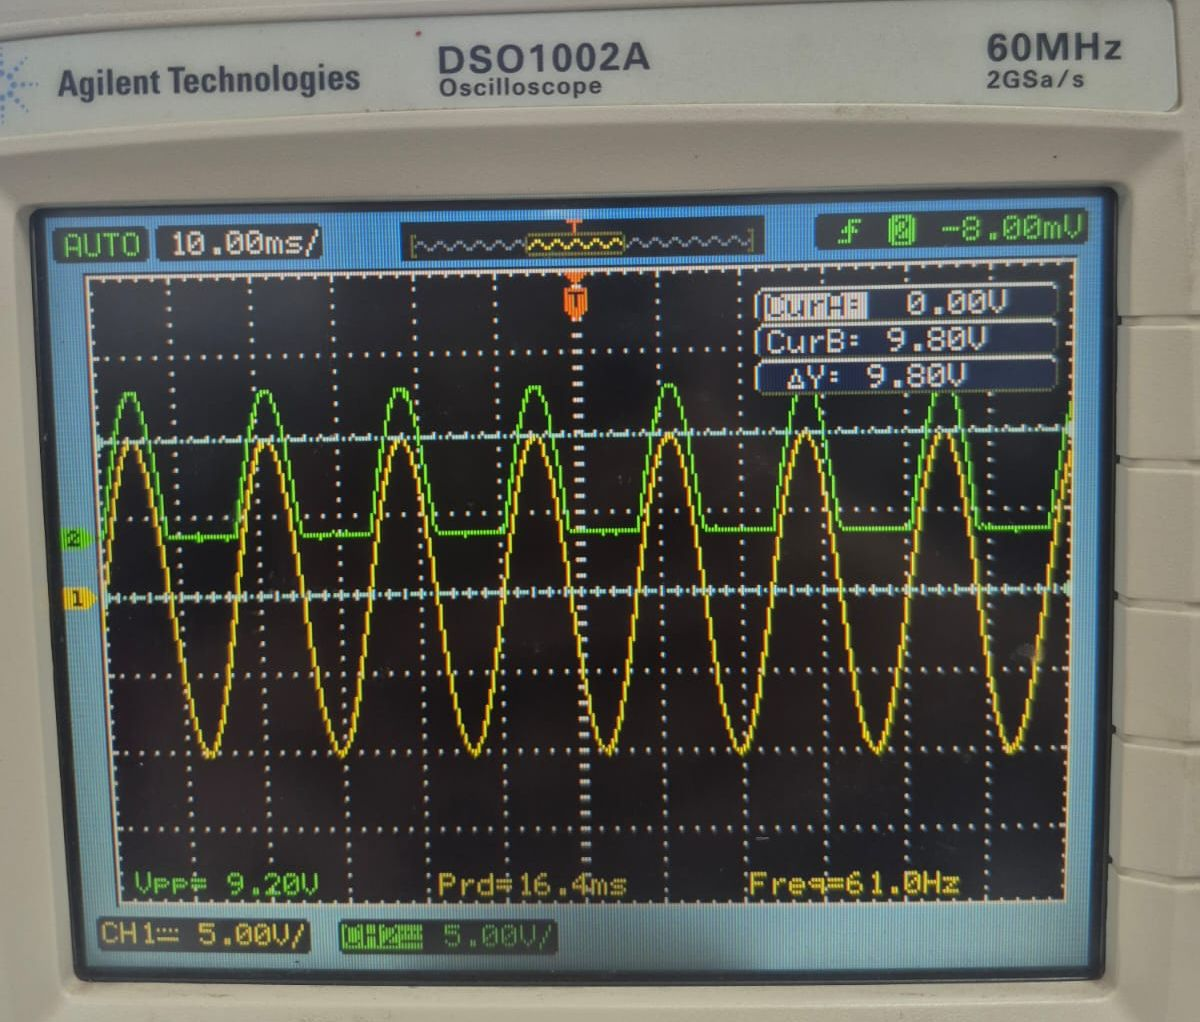
\includegraphics[width=0.8\linewidth]{imagens/ocl_meia_onda.jpg}
  \caption{Leitura do osciloscópio do retificador de meia onda.}
  \label{fig:ocl_meia_onda.jpg}
\end{figure}

\subsubsection{Retificador de meia onda com filtro}
\begin{center}
  \begin{tabular}{@{}lrrrr@{}}
    \toprule
    \textbf{Grandeza} & \textbf{Projeto} & \textbf{Sim. montagem} & \textbf{Medido} &
    \textbf{Erro} \\
    \midrule
		$V_{ripple}$ com capacitor de \SI{47}{\micro\farad}  & \SI{630}{\milli\volt} & \SI{630}{\milli\volt} & \SI{640}{\milli\volt} & 1,5\% \\
		$V_{ripple}$ com capacitor de \SI{4,7}{\micro\farad} & \SI{4,4}{\volt}       & \SI{4,4}{\volt}       & \SI{4,4}{\volt}       & 0\% \\
    \bottomrule
  \end{tabular}
\end{center}

\begin{figure}[H]
  \centering
  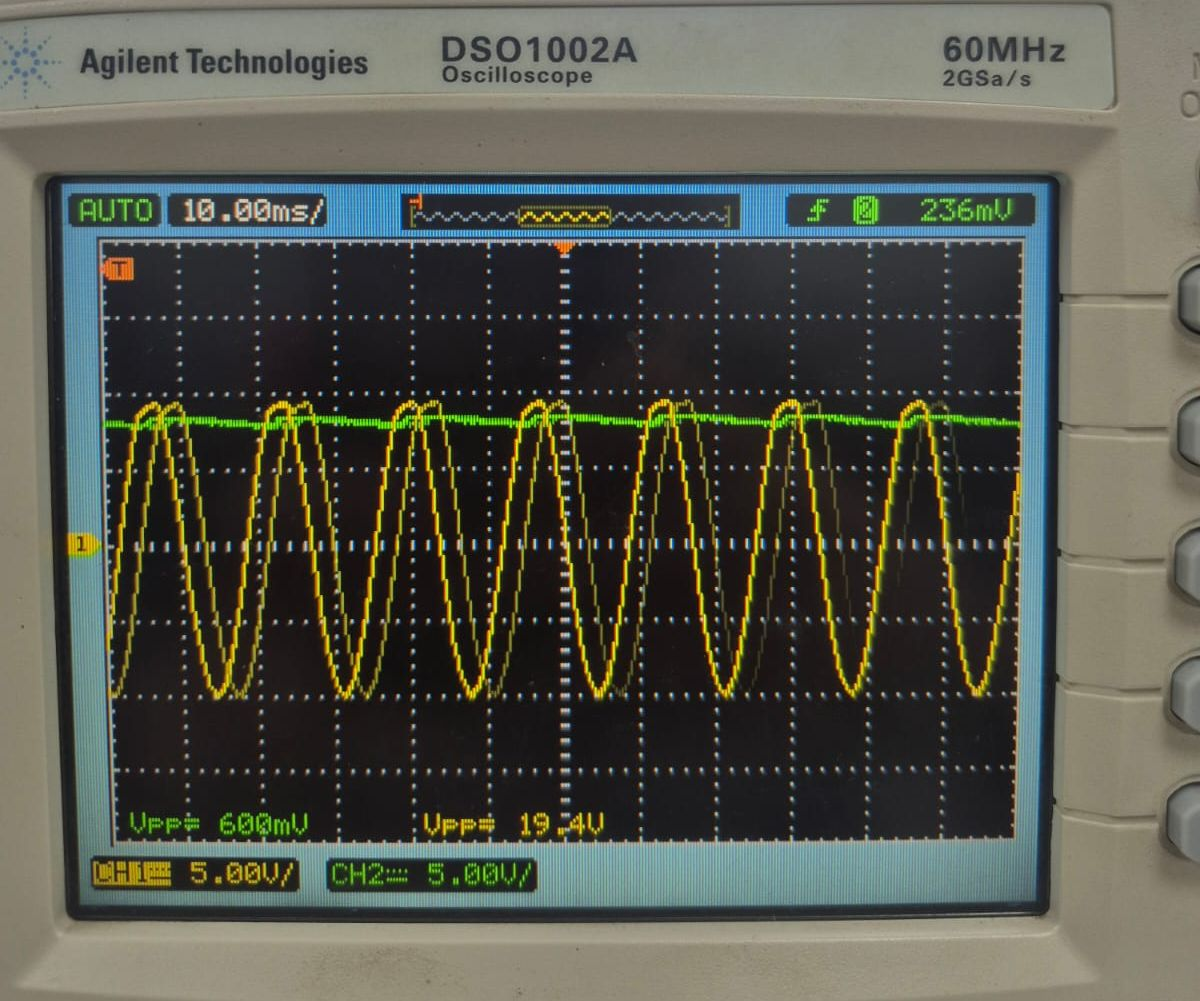
\includegraphics[width=0.8\linewidth]{imagens/ocl_filtro_47_dc.jpg}
  \caption{Leitura do osciloscópio com acoplamento DC na saída do filtro com um capacitor de \SI{47}{\micro\farad}} (meia onda)
  \label{fig:ocl_filtro_47_dc.jpg}
\end{figure}

\begin{figure}[H]
  \centering
  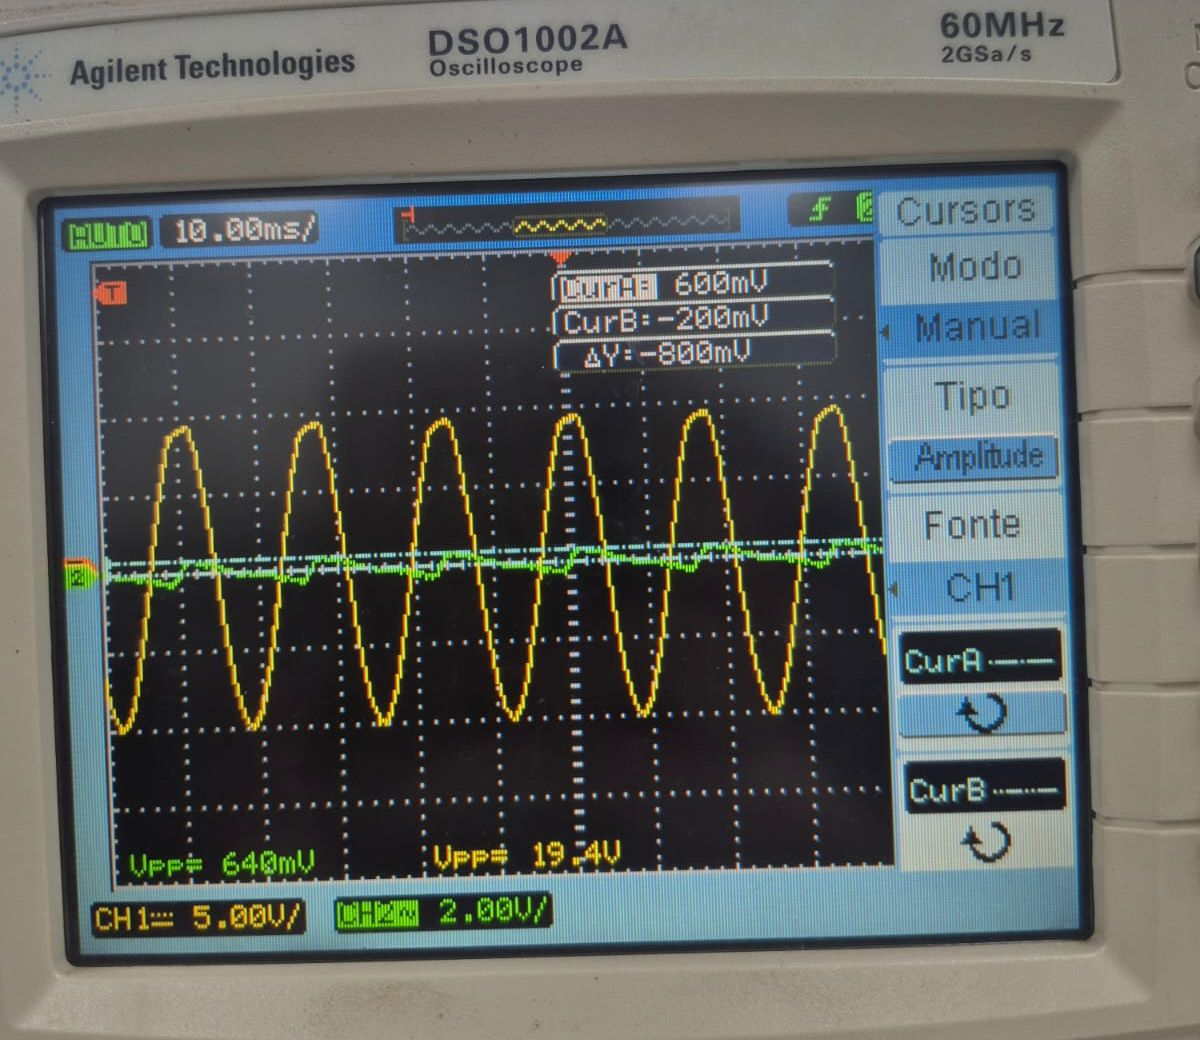
\includegraphics[width=0.8\linewidth]{imagens/ocl_filtro_47_ac.jpg}
  \caption{Leitura do osciloscópio com acoplamento AC na saída do filtro com um capacitor de \SI{47}{\micro\farad}} (meia onda)
  \label{fig:ocl_filtro_47_ac.jpg}
\end{figure}

\begin{figure}[H]
  \centering
  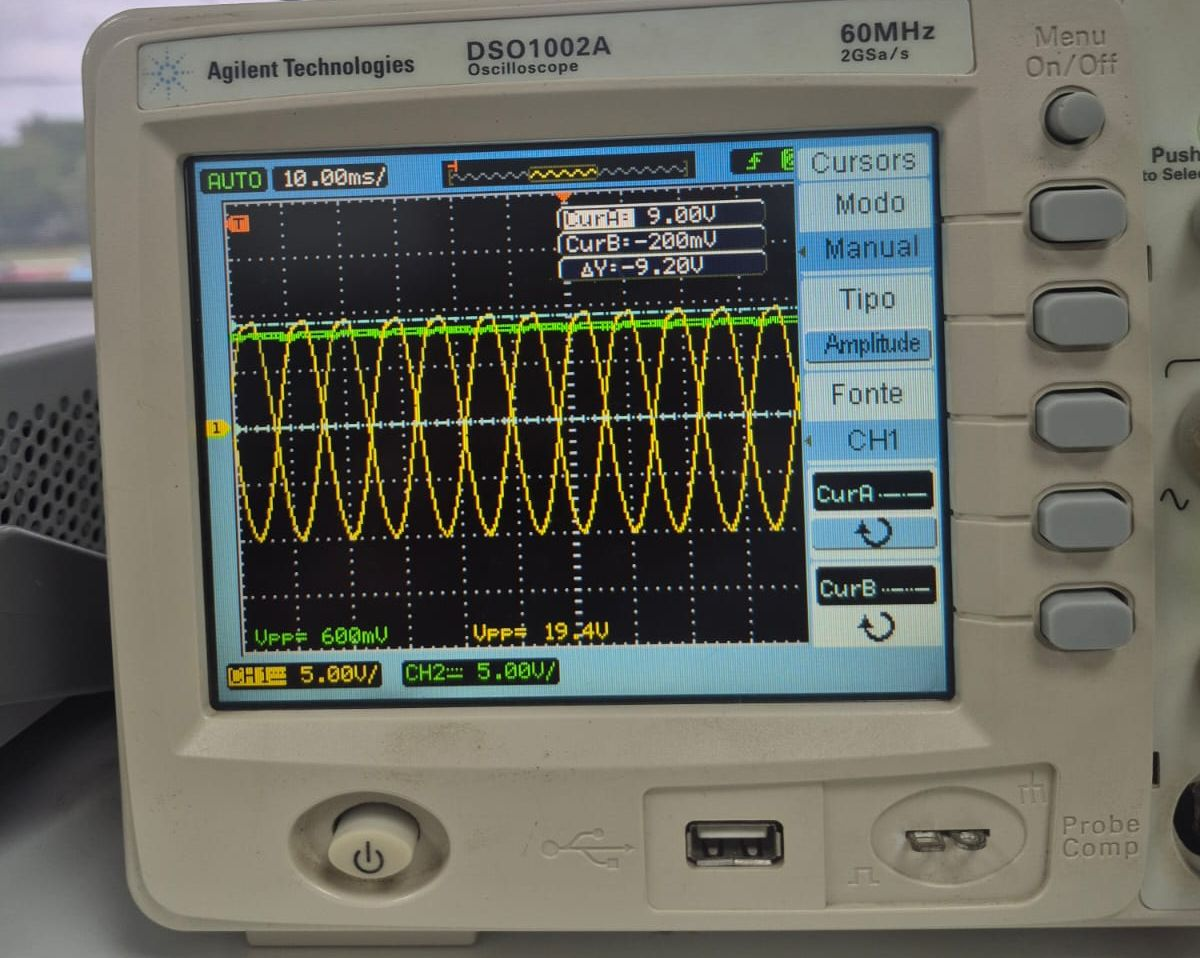
\includegraphics[width=0.8\linewidth]{imagens/ocl_filtro_4,7_dc.jpg}
  \caption{Leitura do osciloscópio com acoplamento DC na saída do filtro com um capacitor de \SI{4.7}{\micro\farad}} (meia onda).
  Esta imagem em particular foi registrada no meio da atualização de quadro do osciloscópio, fazendo a leitura da onda do gerador
  (amarela) aparecer duplicada.
  \label{fig:ocl_filtro_4.7_dc.jpg}
\end{figure}

\begin{figure}[H]
  \centering
  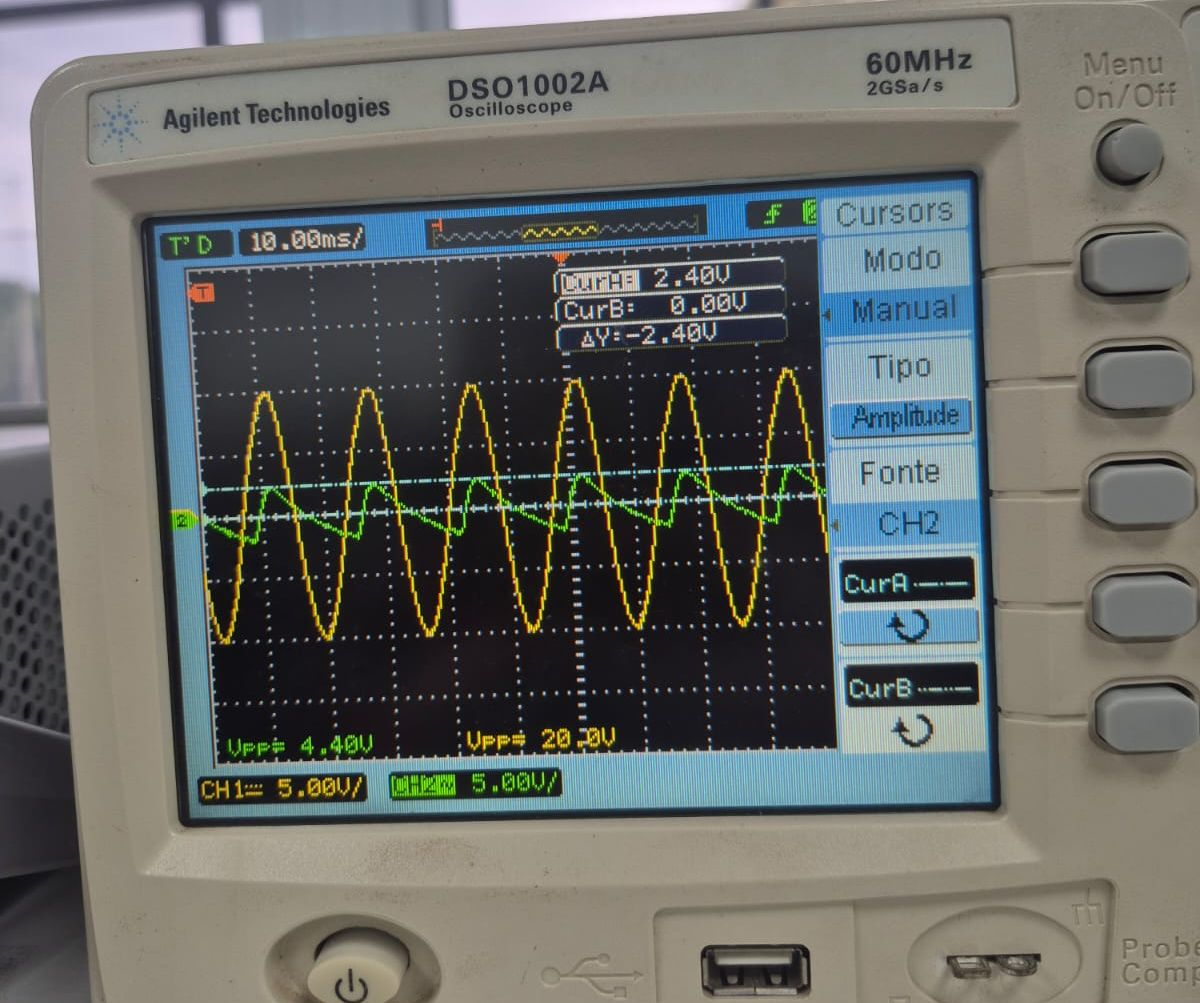
\includegraphics[width=0.8\linewidth]{imagens/ocl_filtro_4,7_ac.jpg}
  \caption{Leitura do osciloscópio com acoplamento AC na saída do filtro com um capacitor de \SI{4.7}{\micro\farad} (meia onda)}
  \label{fig:ocl_filtro_4.7_ac.jpg}
\end{figure}

\subsubsection{Ponte retificadora}
\begin{center}
  \begin{tabular}{@{}lrrrr@{}}
    \toprule
    \textbf{Grandeza} & \textbf{Projeto} & \textbf{Sim. montagem} & \textbf{Medido} &
    \textbf{Erro} \\
    \midrule
		Saída $V_{p}$ da ponte & \SI{8,8}{\volt}  & \SI{8,8}{\volt}  & \SI{8,8}{\volt}   & 0\% \\
    % o que é isso?:
		% $2V_{p}$ da ponte      &                  &                  & \SI{1,025}{\volt} & \\
		Frequência da onda     & \SI{120}{\hertz} & \SI{120}{\hertz} & \SI{119}{\hertz}  & 0,8\% \\
    \bottomrule
  \end{tabular}
\end{center}

\begin{figure}[H]
  \centering
  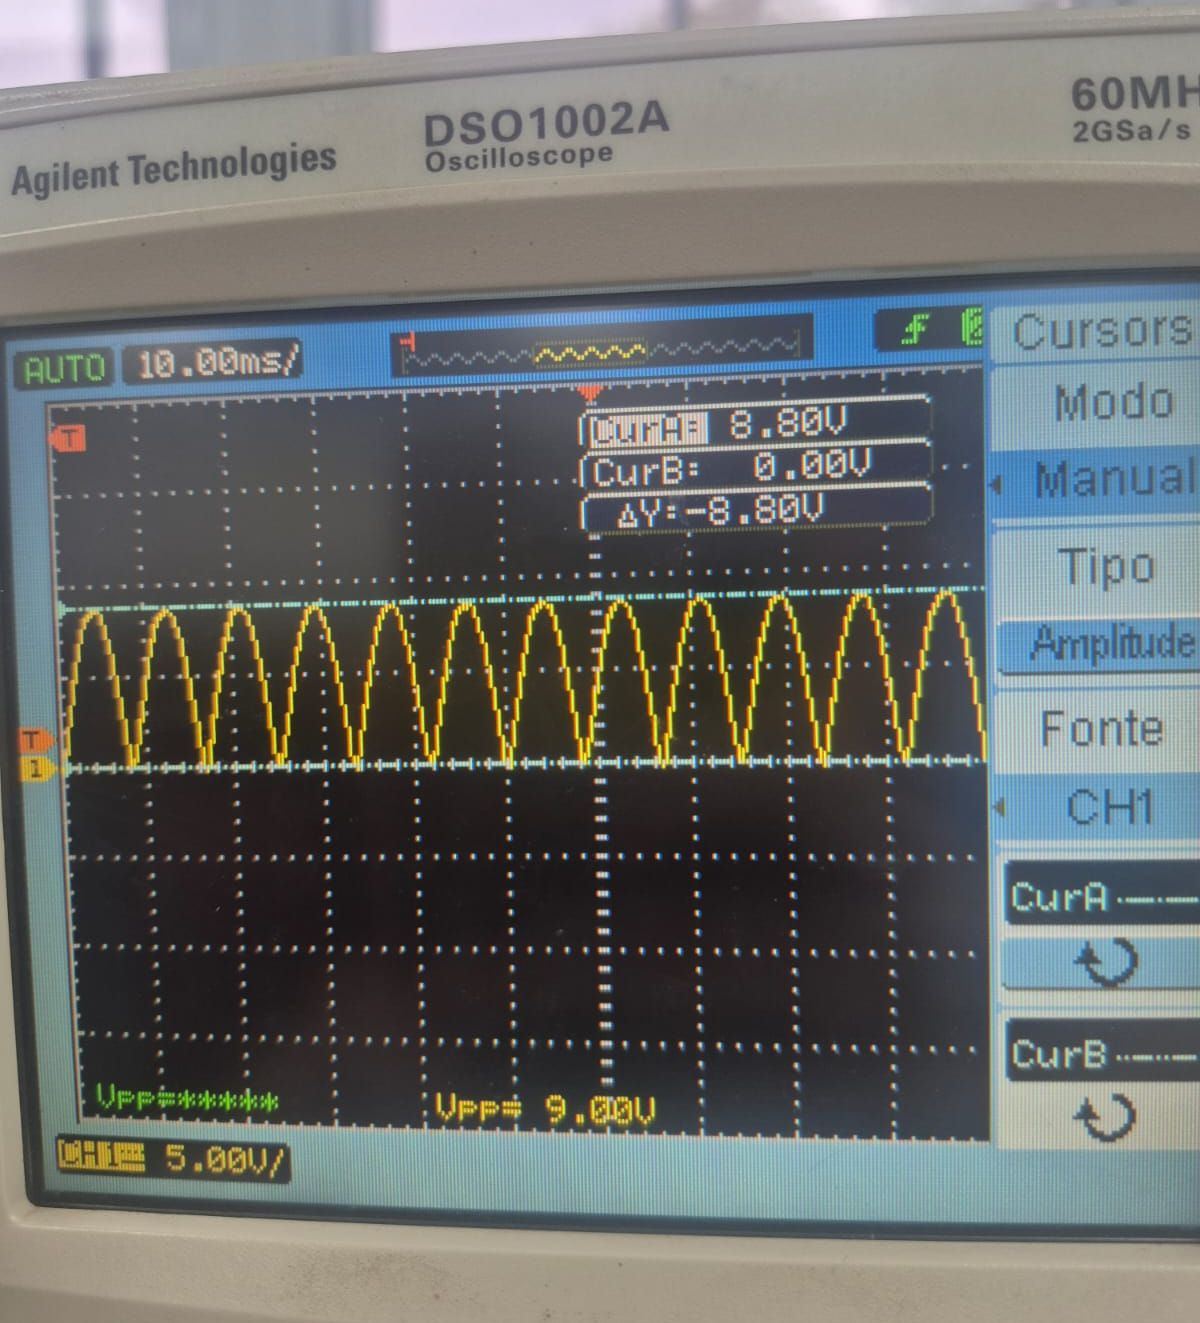
\includegraphics[width=0.8\linewidth]{imagens/ocl_onda_completa.jpg}
  \caption{Leitura do osciloscópio da saída da ponte. É importante notar que não é possível medir a saída da ponte
    e a saída do gerador ao mesmo tempo devido ao fato que o referencial do osciloscópio causar um curto quando
  conectado desta forma.}
  \label{fig:ocl_onda_completa.jpg}
\end{figure}

\subsubsection{Ponte com filtro}
\begin{center}
  \begin{tabular}{@{}lrrrr@{}}
    \toprule
    \textbf{Grandeza} & \textbf{Projeto} & \textbf{Sim. montagem} & \textbf{Medido} &
    \textbf{Erro} \\
    \midrule
		Ripple da ponte com capacitor de \SI{47}{\micro\farad} & \SI{270}{\milli\volt} & \SI{270}{\milli\volt} & \SI{320}{\milli\volt} & 18,5\% \\
		$V_{min}$ & \SI{8,4}{\volt} & \SI{8,4}{\volt} & \SI{7,96}{\volt} & 5,2\% \\
    \bottomrule
  \end{tabular}
\end{center}

\begin{figure}[H]
  \centering
  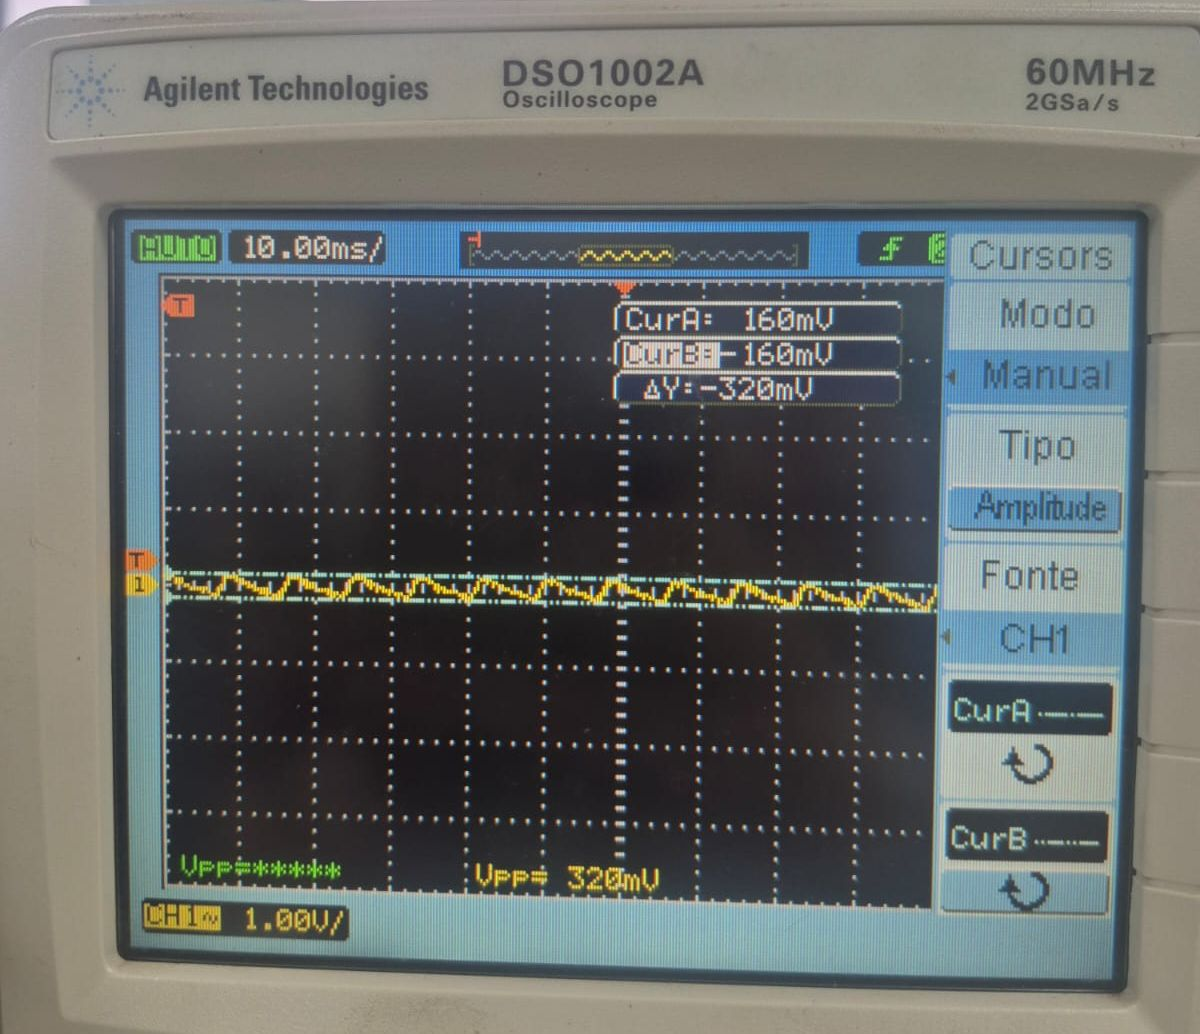
\includegraphics[width=0.8\linewidth]{imagens/ocl_ponte_filtro_ac.jpg}
  \caption{Leitura do osciloscópio com acoplamento AC na saída do filtro com um capacitor de \SI{47}{\micro\farad} (onda completa)}
  \label{fig:ocl_ponte_filtro_ac.jpg}
\end{figure}

\begin{figure}[H]
  \centering
  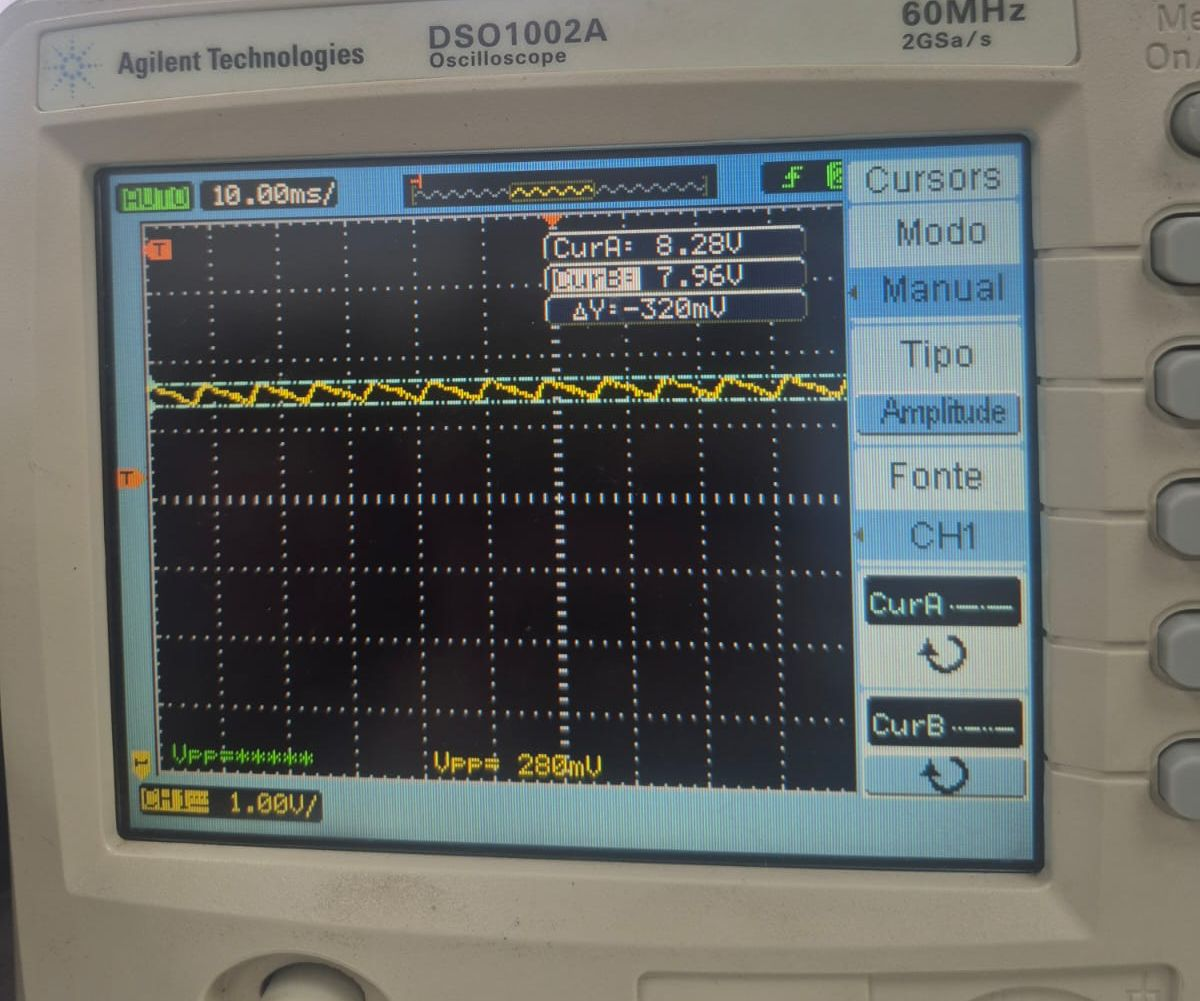
\includegraphics[width=0.8\linewidth]{imagens/ocl_ponte_filtro_dc.jpg}
  \caption{Leitura do osciloscópio com acoplamento DC na saída do filtro com um capacitor de \SI{47}{\micro\farad} (onda completa)}
  \label{fig:ocl_ponte_filtro_dc.jpg}
\end{figure}

\begin{figure}[H]
  \centering
  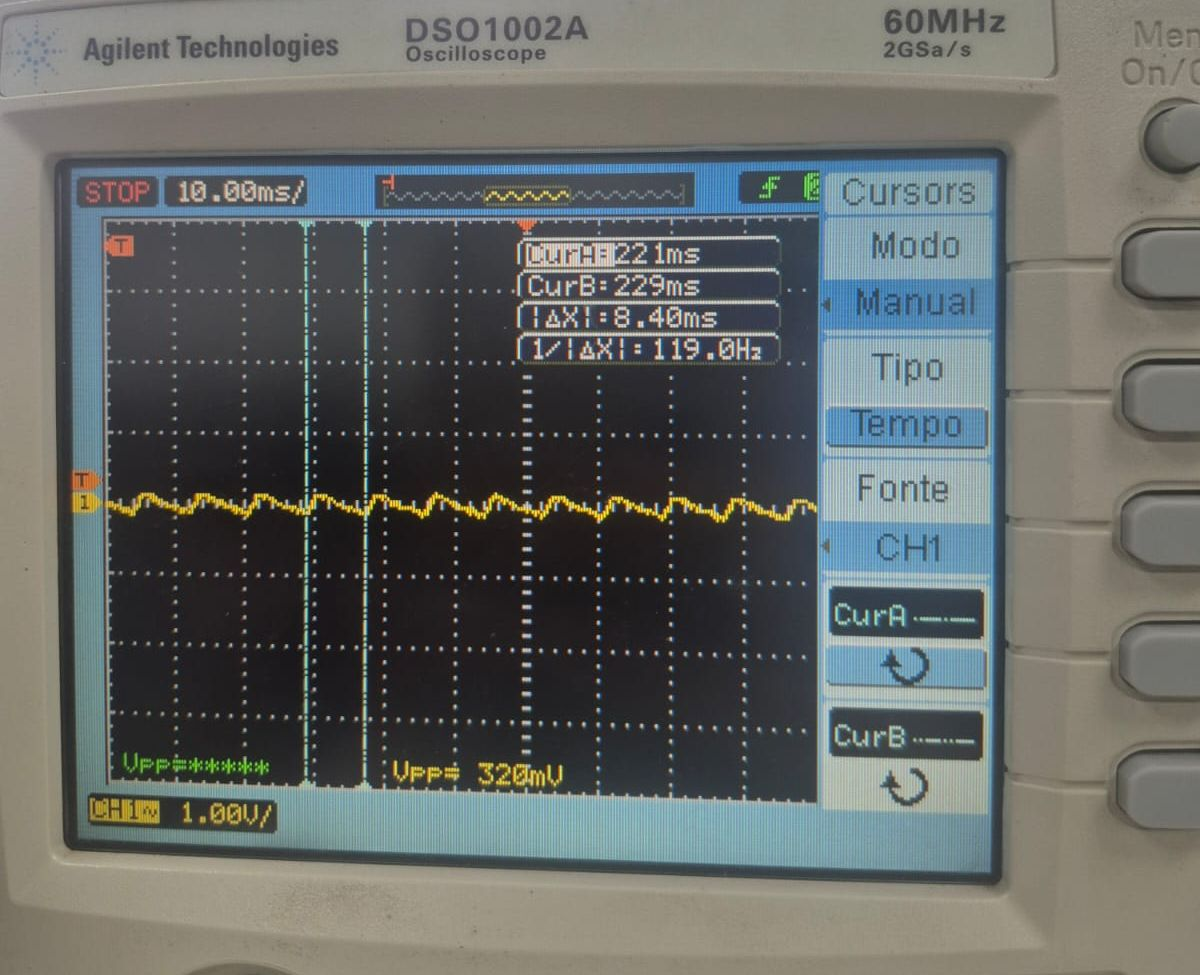
\includegraphics[width=0.8\linewidth]{imagens/ocl_frequencia_ponte.jpg}
  \caption{Leitura do osciloscópio da saída do filtro da ponte usando cursores para medir a frequência. A resolução
  dos cursores do osciloscópio não contempla a frequência exata esperada de \SI{120}{\hertz}, porém chega aos \SI{119}{\hertz}}
  \label{fig:ocl_frequencia_ponte.jpg}
\end{figure}

\subsubsection{Regulação com Zenner}
\begin{center}
  \begin{tabular}{@{}lrrrr@{}}
    \toprule
    \textbf{Grandeza} & \textbf{Projeto} & \textbf{Sim. montagem} & \textbf{Medido} &
    \textbf{Erro} \\
    \midrule
		Saída após regulação & \SI{7,4}{\volt} & \SI{7,4}{\volt} & entre \SI{7,6}{\volt} e \SI{7,2}{\volt} & 2\% \\
    \bottomrule
  \end{tabular}
\end{center}

\begin{figure}[H]
  \centering
  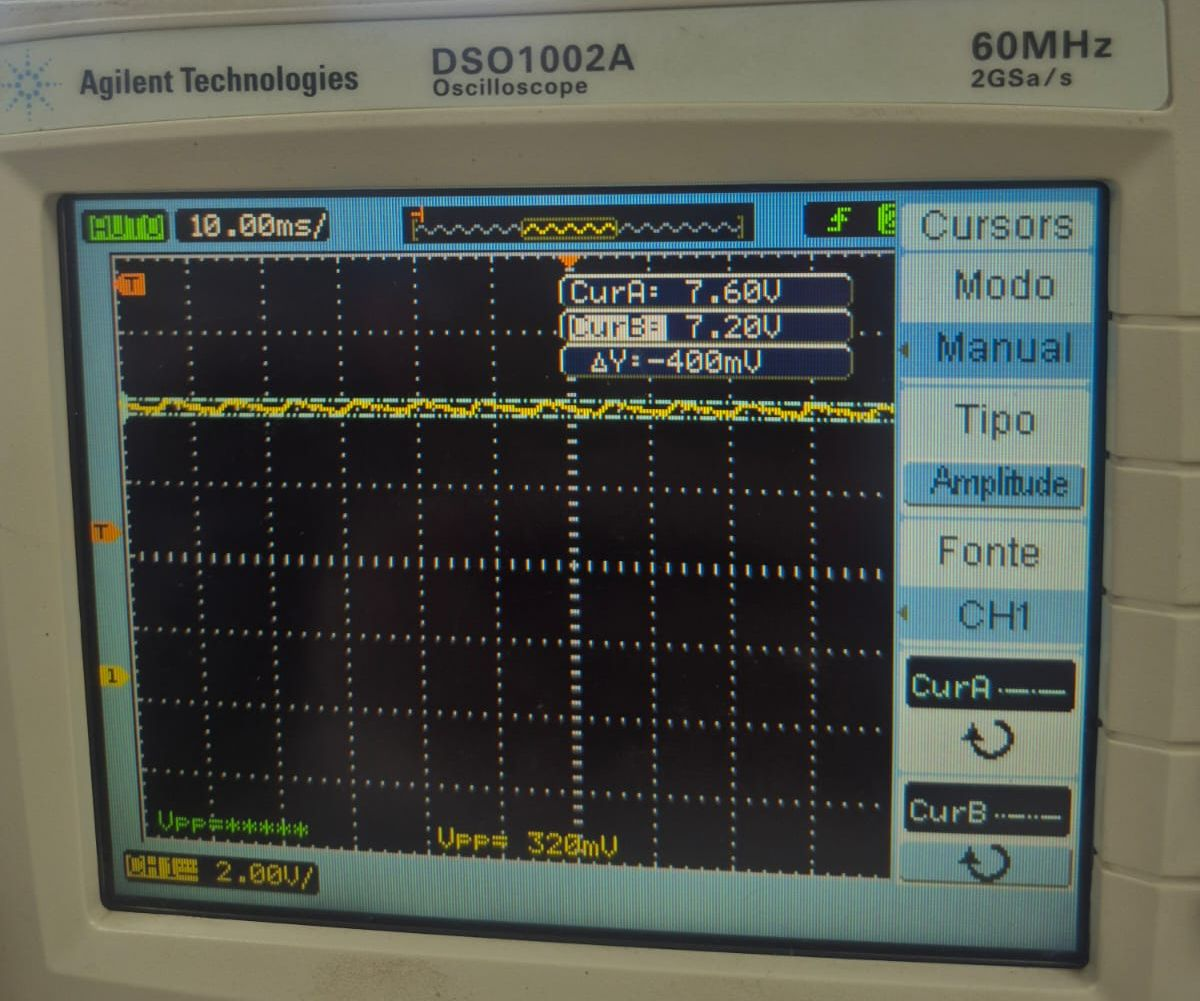
\includegraphics[width=0.8\linewidth]{imagens/ocl_saida_zenner.jpg}
  \caption{Leitura do osciloscópio da saída do regulador com Zenner.}
  \label{fig:ocl_saida_zenner.jpg}
\end{figure}

\section{Discussão}

Percorra as três comparações na ordem em que aparecem no quadro da Seção~4: a conta contra
a simulação de projeto, esta contra a simulação da montagem, e esta contra a medição. Cada
passo isola uma causa, e a discussão fica bem mais curta quando eles não se misturam.

Compare também os projetos dos integrantes entre si. Como as especificações são diferentes,
os resultados diferem, e mostrar que essa diferença é a que a teoria previa vale mais do
que repetir três vezes a mesma análise.

Sempre que uma divergência for maior do que a incerteza esperada, aponte uma causa concreta
e diga como ela poderia ser reduzida. Vale, por exemplo, a tolerância do componente, a
resistência série do indutor, a impedância de entrada do osciloscópio, a banda do
amplificador ou a resolução da varredura.

Quando previsto e obtido coincidirem, explique por que era esperado que coincidissem, e o
que essa coincidência não permite concluir.

Por fim, retome as hipóteses que vocês declararam na fundamentação e diga quais se
confirmaram. Se algo observado contrariar a previsão, resolva a contradição aqui.

\section{Conclusão}

Retome o objetivo que vocês anunciaram na introdução e responda se ele foi atingido,
apoiando a resposta em um número. Aponte a principal limitação do que foi feito e o que
ela impede de afirmar. Evite trazer resultado novo nesta seção.

\section{Referências}

\begin{referencias}
\item SEDRA, A.~S.; SMITH, K.~C. \emph{Microeletrônica}. 5.~ed. São Paulo: Pearson
  Prentice Hall, 2007.
\item BOYLESTAD, R.~L.; NASHELSKY, L. \emph{Dispositivos Eletrônicos e Teoria de
  Circuitos}. 11.~ed. São Paulo: Pearson Education do Brasil, 2013.
\end{referencias}

\end{document}
